\documentclass[12pt]{article}
\usepackage{geometry}
\geometry{a4paper, bottom=40mm, top=40mm, left=25mm, right=25mm}
\usepackage{pdfpages}
\usepackage{fancyhdr}
\pagestyle{fancy}
\setlength{\parindent}{0cm}
\setlength{\headheight}{14pt}
\usepackage{tocloft}
\usepackage{parskip}
\usepackage[export]{adjustbox}
\usepackage{float}
\usepackage{subfig}
\usepackage{graphicx}
\graphicspath{{../figures}}
\usepackage{amsmath,blkarray,booktabs,bigstrut, amssymb}
\usepackage{pythonhighlight}
\usepackage{outlines}
\usepackage[hidelinks]{hyperref}
\usepackage[backend=biber, style=ieee]{biblatex}
\addbibresource{references.bib}
% \bibliographystyle{ieee} % or another style like IEEE, APA, etc.
% \nocite{*}
\usepackage{url}
\setcounter{biburllcpenalty}{7000}
\setcounter{biburlucpenalty}{8000}
\widowpenalty10000
\clubpenalty10000
\setcounter{secnumdepth}{0}
\usepackage[newfloat]{minted}
\usepackage{caption}
\newenvironment{code}{\captionsetup{type=listing}}{}
\SetupFloatingEnvironment{listing}{name=Code Listing}


\begin{document}

\newgeometry{top=20mm}
\begin{titlepage}
    \begin{center}
      \begin{figure}
        
\includegraphics[right]{logo.png}
      \end{figure}
      \vspace*{1cm}
      \textsc{\large ENEL373: Digital Electronics and Devices}\\[0.5cm]
      \textsc{\Large University of Canterbury}\\[3.5cm]
      \linespread{1}
      {\Huge\bfseries This is an Awesome Title \\[0.3cm] for Our First Report} \\
      \vspace*{2cm}
      {\Huge Philip Brand \textit{\Large(15776928)}\\\par}
      % ADD YOUR NAME AND STUDENT ID HERE
      \vspace*{3cm}
      {\LARGE \today}
    \end{center}
  \end{titlepage}
\restoregeometry

\fancyhead{}
\fancyhead[L]{\small{ENEL373 - Reaction Timer Project}}
\fancyhead[R]{\small{\today}}

\pagenumbering{roman}

% \addcontentsline{toc}{section}{Abstract}
% \section*{Abstract}

% Not sure if we need an abstract

% \newpage

\renewcommand{\baselinestretch}{1.3}\normalsize
\setlength{\cftbeforesecskip}{0.3em}
\renewcommand{\cftsecleader}{\cftdotfill{\cftdotsep}}
\addcontentsline{toc}{section}{Contents}
\tableofcontents\thispagestyle{fancy}
\renewcommand{\baselinestretch}{1}\normalsize

\newpage
\pagenumbering{arabic}

\section{Introduction}
% Outline (in your own words) the project requirements and what you achieved

Human reaction time is the interval between the a stimulus and the response to that stimulus. There are two main types of reaction time; simple, and choice. Simple reaction involves reacting to a singular stimulus, while choice reaction involves choosing the correct response from multiple stimuli. This project aims to implement a simple reaction time recorder on an FPGA in VHDL.

The reaction stimulus is three LEDs that turn off sequentially, with a random delay between each LED turning off. Once the last LED turns off, the user must press a button, and the delay is displayed in milliseconds on 8 7-segment displays. The FPGA stores the reaction delays from the last three trials, and can display the fastest, slowest, and average reaction times. These values can be reset by the user.

\section{Design Summary}
% Summarise your design.


\newpage

\section{Design Details}
% (~2 pages): Describe the methods your group used to implement your FPGA design. Justify your final design. Support your descriptions and justifications with specific, explicit references to your VHDL source code in the appendix. VHDL descriptions could, for example, include an RTL description. 

% PHILIP says - is it worth including a state diagram for the FSM?

\subsection{Finite State Machine}

The reaction timer was managed by a finite state machine with the following states: (change these to match the ones in the code)
\begin{itemize}
    \item \textbf{Idle}: The system is waiting for the user to press the start button. The LEDs are on, and the 7-segment displays are blank.
    \item \textbf{Countdown}: The system is counting down from a random number between 1 and 5 seconds. The LEDs are off, and the 7-segment displays are blank.
    \item \textbf{Reaction}: The system is waiting for the user to press the button after the last LED turns off. The LEDs are off, and the 7-segment displays are blank.
    \item \textbf{Display}: The system is displaying the reaction time on the 7-segment displays. The LEDs are off, and the 7-segment displays show the reaction time in milliseconds.
    \item \textbf{Store}: The system is storing the reaction time in the memory. The LEDs are off, and the 7-segment displays are blank.
    \item \textbf{Reset}: The system is resetting the memory. The LEDs are off, and the 7-segment displays are blank.
\end{itemize}

The reaction delays were stored in a three-element circular buffer.

\subsection{Pseudo-Random Number Generation}

The pseudo-random delay between the sequential deactivation of the LEDs was generated using a linear feedback shift register (LFSR) and a clock divider. An eight-bit LFSR was used to generate pseudo-random numbers, and a selection of those bits were assigned to the most significant eight bits of the upper bound for the clock divider. The next pseudo-random number was generated on a rising clock edge from that clock divider, as seen in Listing \ref{code:random_number_generation}.

\begin{code}
\begin{minted}{vhdl}

--  Generate next "random" number from the LFSR in random_number_generator
  ff9: random_number_generator port map (CLK_IN => clk_var_hz,
                                         RAND_OUT => rand_num);
  
-- Set the upperbound for the variable clk based on the random number  
  clk_var_hz_divider_bound(27 downto 20) <= rand_num;

-- Generate another clk square wave to trigger a new random number
  ff10: clk_divider port map(CLK100MHZ_IN => CLK100MHZ,
                              SLOWCLK_OUT => clk_var_hz,
                              UPPERBOUND_IN => clk_var_hz_divider_bound);
\end{minted}
\captionsetup{belowskip=0pt}
\captionof{listing}{Behavioural VHDL implementation of pseudo-random number generation.}
\label{code:random_number_generation}
\end{code}

If all eight bits of the LFSR set the most significant bits of the upper bound, the minimum delay between LEDs turning off would be,

\[
\text{Minimum Delay} = \frac{2^{20} - 1}{100 \text{ MHz}} = 11 \text{ ms}.
\]

It was decided this would be too short a delay. Instead of reducing the number of bits in the LFSR, the four most significant bits of the upper bound were set by the middle four bits of the LFSR. This increased the minimum delay to,

\[
\text{New Minimum Delay} = \frac{2^{24} - 1}{100 \text{ MHz}} = 167\text{ ms},
\]

which was acceptable. The maximum delay remained unchanged, at

\[
\text{Maximum Delay} = \frac{2^{28} - 1}{100 \text{ MHz}} = 2.68 \text{ s}.
\]

The location of the taps in the LFSR were chosen to ensure a maximum period of $2^8 - 1 = 255$ cycles. These locations were 8, 6, 5, and 4 \cite{lfsr_taps}, as seen in Listing \ref{code:lfsr}.

\begin{code}
\begin{minted}{vhdl}

  process (CLK_IN)
  begin
      if rising_edge(CLK_IN) then
          current_rand(7 downto 1) <= current_rand(6 downto 0);
          current_rand(0) <= current_rand(7) XOR current_rand(5) ...
          ... XOR current_rand(4) XOR current_rand(3);
      end if;
  end process;

  RAND_OUT <= current_rand;
\end{minted}
\captionsetup{belowskip=0pt}
\captionof{listing}{Dataflow VHDL implementation of LFSR.}
\label{code:lfsr}
\end{code}

\subsection{8-1 mux}


\subsection{ALU \& Circular Buffer}


\subsection{Text Override}



\newpage

\section{Module Testing}
% A brief section describing how you tested a significant module. Include at least one testbench and associated waveforms that demonstrate the functionality of a module in the report appendix.

\newpage

\section{Conclusions}
% Highlight any problems you encountered and how you solved them. Also discuss what you learned and give suggestions on how the project could be improved


\newpage
% There is no need to include a full code listing in your report as your code will be submitted via eng-git. However, reference to a code snippet in an appendix is quite appropriate. Formal citations to books, web articles, open source VHDL code and other sources should be listed in a reference section that uses the IEEE style and format.


\printbibliography

\newpage
\appendix

Here is how we include a figure in the report. Figure \ref{fig:example} shows an example of a figure. A figure.

\begin{figure}[H]
  \centering
  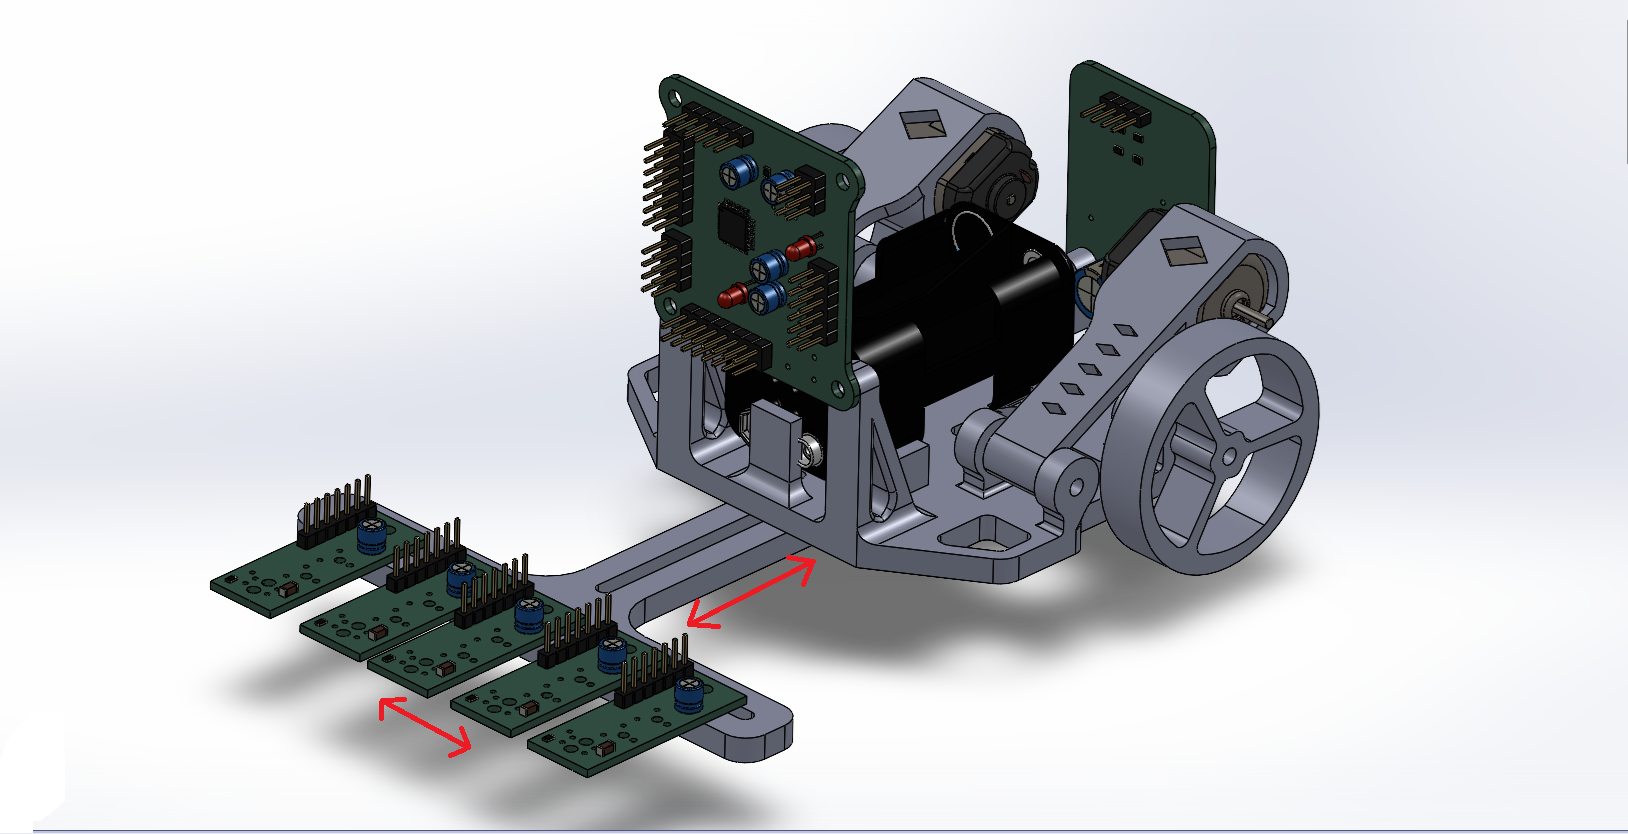
\includegraphics[width=0.8\textwidth]{example.png}
  \caption{This is an example of a figure.}
  \label{fig:example}
\end{figure}


\end{document}
